\thispagestyle{duongvaotoanhocnone}
\pagestyle{duongvaotoanhoc}
\everymath{\color{duongvaotoanhoc}}
\graphicspath{{../duongvaotoanhoc/pic/}}
\blfootnote{$^1$\color{duongvaotoanhoc}Universit\'e Paris--Saclay.}
\begingroup
\AddToShipoutPicture*{\put(0,616){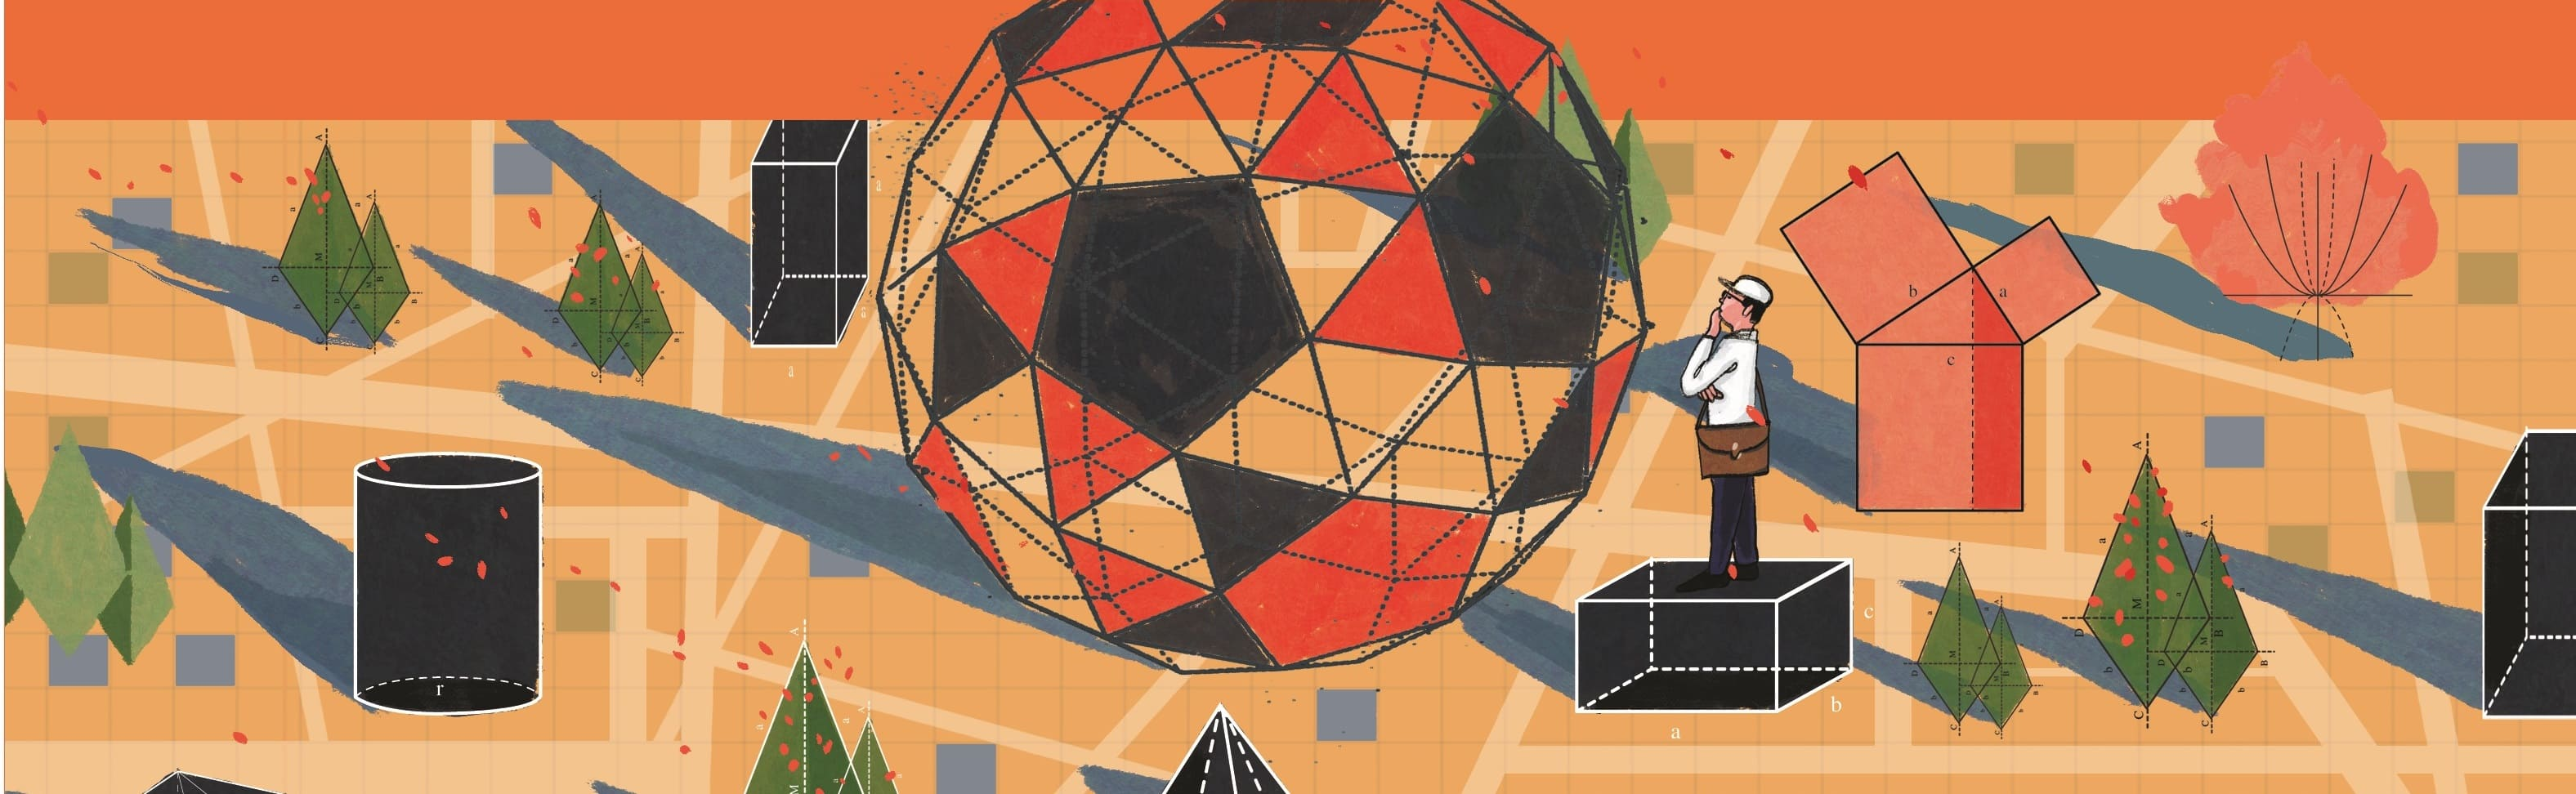
\includegraphics[width=19.3cm]{../bannerduongvao}}}
\AddToShipoutPicture*{\put(84,523){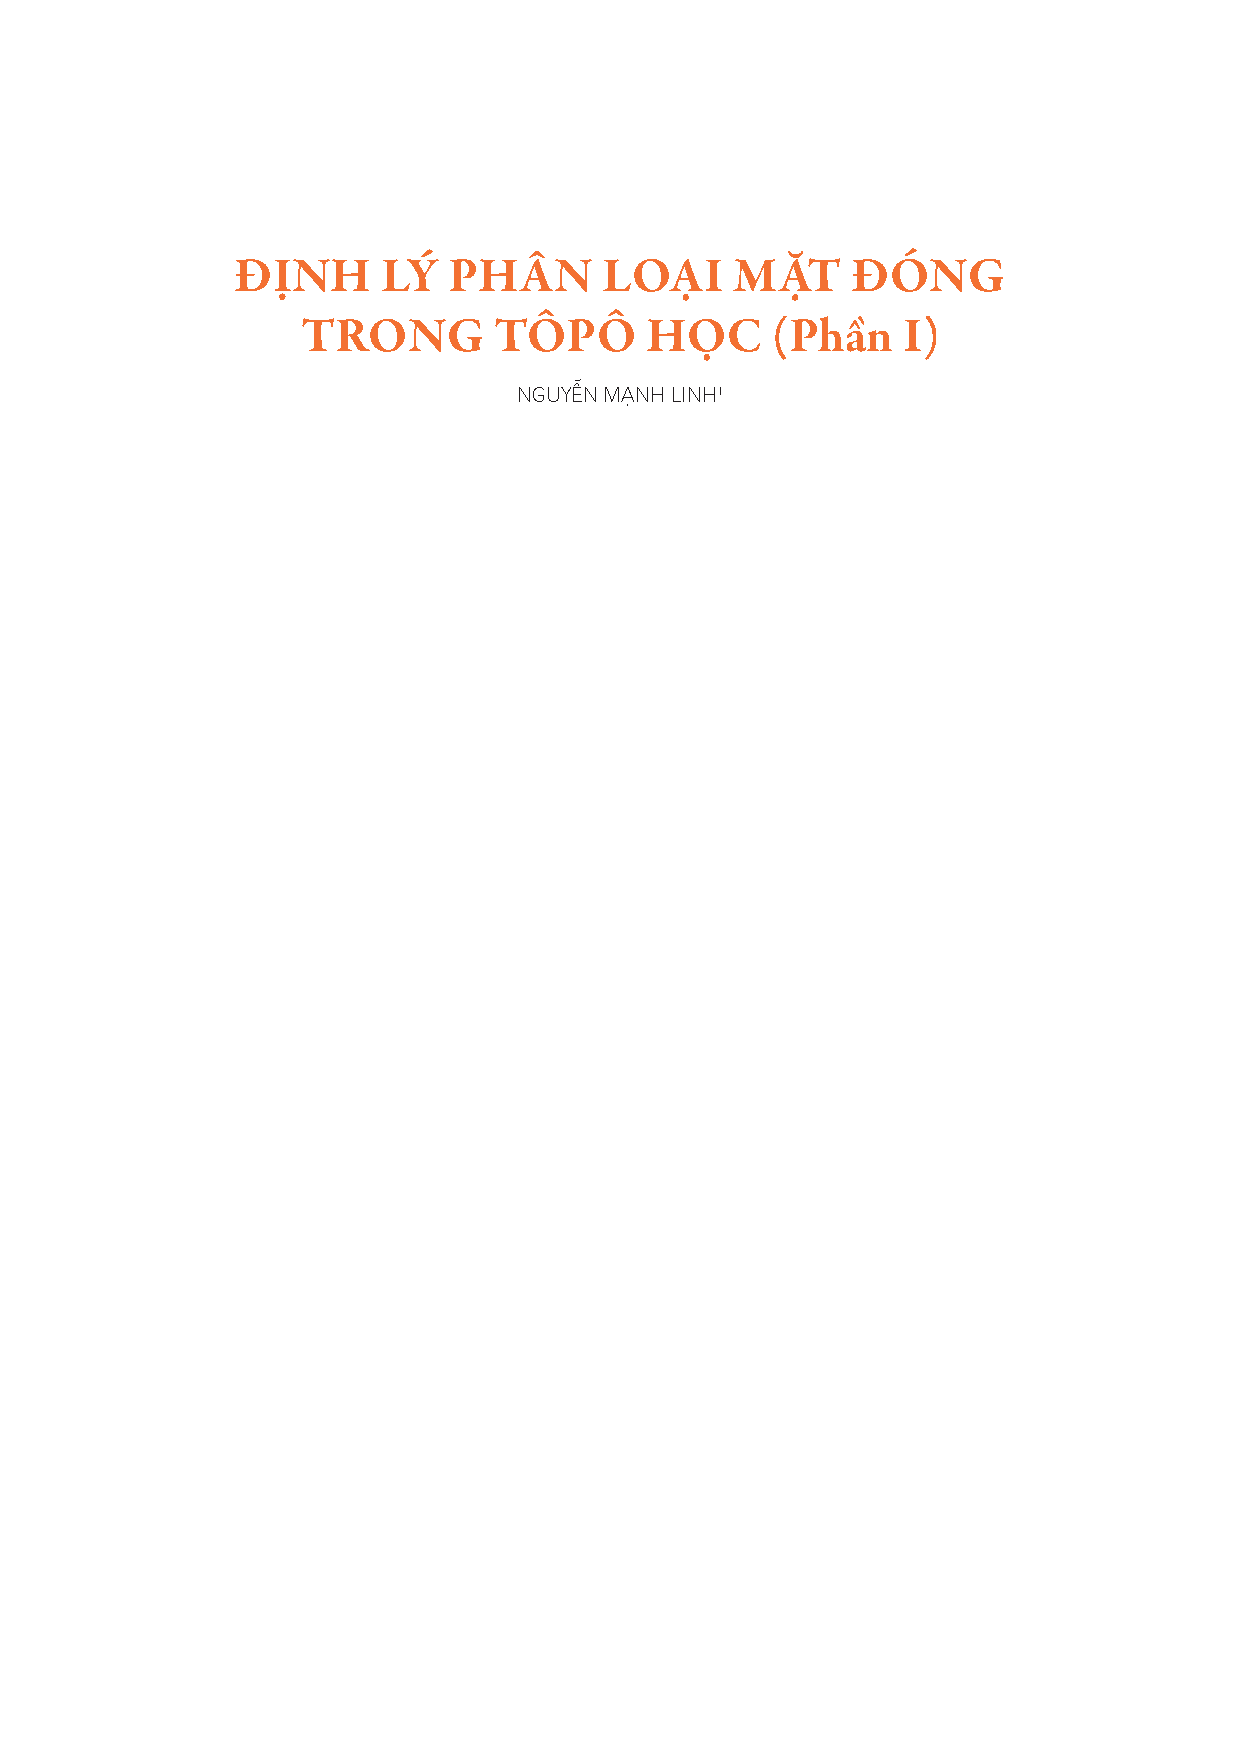
\includegraphics[scale=1]{../tieude.pdf}}}
\centering
\endgroup
\vspace*{185pt}

\begin{multicols}{2}	
	Định lý phân loại mặt đóng có lẽ là một trong những định lý cơ bản nhất của tôpô học. Trong ghi chú này, chúng ta giới thiệu và ``chứng minh'' định lý này một cách trực quan, bằng kiến thức toán học tối thiểu.
	\vskip 0.1cm
	$\pmb{1.}$ \textbf{\color{duongvaotoanhoc}Một số định nghĩa tôpô}
	\vskip 0.1cm
	{\it Tôpô học} là lĩnh vực toán học nghiên cứu các hình dạng mà không quan tâm đến các đặc tính như khoảng cách hay diện tích... Thay vào đó, người ta quan tâm đến các đặc tính nội tại bất biến dưới các phép biến dạng liên tục nhưng không xé rách hay dán các hình dạng đó (các {\it tính chất tôpô}). Đối tượng làm việc của tôpô học là các {\it không gian tôpô}, đó là những tập hợp cùng với một cấu trúc cho phép ta nói về khái niệm gần nhau của các điểm cũng như khái niệm {\it lân cận} (nhưng không nhất thiết phải đo được khoảng cách giữa các điểm).
	\vskip 0.1cm
	Cho $X$ là một không gian tôpô và $x \in X$ là một điểm. Nói chung, một lân cận của $x$ trong $X$ không phải là một tập con chứa $x$ bất kỳ của $X$. Đối với các không gian tôpô thông thường (chẳng hạn, trong toàn bộ ghi chú này), ta sẽ hiểu một cách không chính thức rằng một tập con $U \subset X$ là một lân cận của $x$ nếu $x \in U$ và ta có thể ``di chuyển một cách tự do theo tất cả các hướng'' xung quanh $x$ một khoảng đủ nhỏ sao cho vẫn nằm trong $U$. Chẳng hạn, với $X = \mathbb{R}$ là đường thẳng thực, một tập con $U \subset \mathbb{R}$ là một lân cận của một số thực $x$ nếu nó chứa một khoảng $(x - \varepsilon, x + \varepsilon)$, với $\varepsilon > 0$ đủ nhỏ nào đó (xem Hình $1$).
	\begin{figure}[H]
		\vspace*{-5pt}
		\centering\captionsetup{labelformat=empty, justification=centering}
		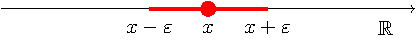
\includegraphics[width=1\linewidth]{H1.pdf}
		\caption{\small\textit{\color{duongvaotoanhoc}Hình $1$: Lân cận của một điểm $x \in \mathbb{R}$.}}
		\vspace*{-10pt}
	\end{figure}
	Định nghĩa sau đây sẽ đóng vai trò trung tâm trong việc xây dựng khái niệm mặt. Trong mặt phẳng $\mathbb{R}^2$, ta có khoảng cách giữa hai điểm $\mathbf{x} = (x_1,x_2)$ và $\mathbf{y} = (y_1,y_2)$, cho bởi công thức
	\begin{align*}
		\left\|\mathbf{x} - \mathbf{y}\right\| = \sqrt{(x_1 - y_1)^2 + (x_2 - y_2)^2}.
	\end{align*}
	Ta định nghĩa {\it đĩa mở} với tâm $\mathbf{x} \in \mathbb{R}^2$ và bán kính $r > 0$ bởi
	\begin{align*}
		\mathbb{D}(\mathbf{x}, r) = \{ y \in \mathbb{R}^2:  \left\|\mathbf{x} - \mathbf{y}\right\| < r\}
	\end{align*}
	(đó là hình tròn tâm $\mathbf{x}$ bán kính $r$ không kể biên), cũng như {\it đĩa đóng} tâm $\mathbf{x}$ bán kính $r$ bởi
	\begin{align*}
		\overline{\mathbb{D}}(\mathbf{x}, r) = \{ y \in \mathbb{R}^2:  \left\|\mathbf{x} - \mathbf{y}\right\| \le r\}
	\end{align*}
	(đó là hình tròn tâm $\mathbf{x}$ bán kính $r$ kể cả biên). Với $\mathbf{x} = (0,0)$ là gốc tọa độ và $r = 1$, ta sẽ ký hiệu đơn giản $\mathbb{D} = \mathbb{D}((0,0),1)$, $\overline{\mathbb{D}} = \overline{\mathbb{D}}((0,0),1)$ và gọi chúng lần lượt là {\it đĩa mở đơn vị} và {\it đĩa đóng đơn vị}. Xét không gian $X = \overline{\mathbb{D}}$. Với $\mathbf{x} \in \mathbb{D}$, một tập con của $\overline{\mathbb{D}}$ là một lân cận của $\mathbf{x}$ nếu nó chứa một đĩa $\mathbb{D}(\mathbf{x},r)$ với $r > 0$ đủ nhỏ. Tuy nhiên, với $\mathbf{x} \in \overline{\mathbb{D}} \setminus \mathbb{D}$, một tập con của $\overline{\mathbb{D}}$ là một lân cận của $\mathbf{x}$ nếu nó chứa phần giao của một đĩa như vậy với $\overline{\mathbb{D}}$, giao này không phải là một đĩa (xem Hình $2$).
	\begin{figure}[H]
		\vspace*{-5pt}
		\centering\captionsetup{labelformat=empty, justification=centering}
		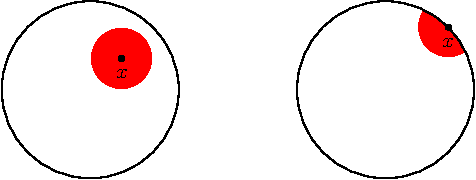
\includegraphics[width=1\linewidth]{H2.pdf}
		\caption{\small\textit{\color{duongvaotoanhoc}Hình $2$: Lân cận trong $\overline{\mathbb{D}}$ của một điểm $\mathbf{x} \in \mathbb{D}$ và một điểm $\mathbf{x} \in \overline{\mathbb{D}} \setminus \mathbb{D}$.}}
		\vspace*{-10pt}
	\end{figure}
	Đẳng thức là một khái niệm cơ bản của toán phổ thông, nó thể hiện sự đồng nhất tuyệt đối. Tuy nhiên, khi định nghĩa các đối tượng toán học có cấu trúc phức tạp hơn (các không gian tôpô chẳng hạn), để nói về sự giống nhau giữa chúng thì ``bằng nhau'' là một đòi hỏi quá đáng. Nó được thay bởi một định nghĩa rộng hơn là {\it đẳng cấu}, có thể hiểu là ``về cơ bản là bằng nhau''. Trong ngữ cảnh của các không gian tôpô, sự đẳng cấu được thể hiện qua các {\it phép đồng phôi}. Trước hết, một ánh xạ $f: X \to Y$ giữa hai không gian tôpô được gọi là {\it liên tục} nếu với mỗi $x \in X$ và mỗi lân cận $V \subset Y$ của $f(x)$, tồn tại lân cận $U \subset X$ sao cho $f(U) \subset V$. Nói cách khác, khi $y$ thay đổi trên $X$, điểm $f(y)$ có thể gần (nằm trong lân cận nhỏ tùy ý của) $f(x)$, miễn là $y$ đủ gần $x$. Ta gọi $f$ là một {\it phép đồng phôi} nếu nó là một song ánh và ánh xạ ngược $f^{-1}: Y \to X$ cũng liên tục. Nếu tồn tại một phép đồng phôi như vậy, ta nói $X$ và $Y$ {\it đồng phôi (với nhau)} và viết $X \approx Y$. Ta có thể hiểu một phép đồng phôi là một biến dạng liên tục có thể đảo ngược: không xé rách, không dán... không gian tôpô ban đầu (và quá trình đảo ngược cũng là một biến dạng liên tục). Các thuộc tính của không gian tôpô được bảo toàn bởi các phép đồng phôi được gọi là các {\it bất biến tôpô}.
	\vskip 0.1cm
	Chẳng hạn, trong mặt phẳng, xét (biên của) hình vuông đơn vị cho bởi phương trình $\max\{|x|,|y|\} = 1$ cũng như đường tròn đơn vị cho bởi phương trình $x^2 + y^2 = 1$. Chúng đồng phôi với nhau bởi ánh xạ liên tục ở Hình $3$.
	\begin{figure}[H]
		\vspace*{-5pt}
		\centering\captionsetup{labelformat=empty, justification=centering}
		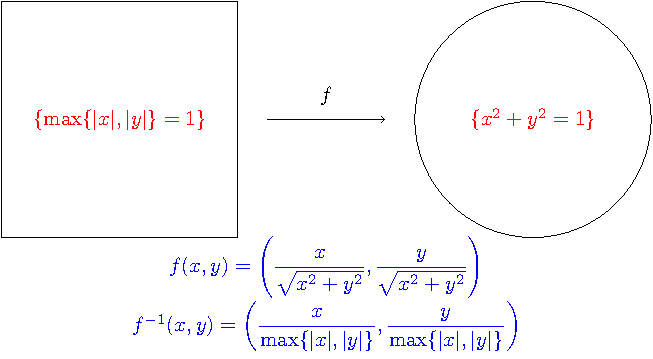
\includegraphics[width=1\linewidth]{H3.pdf}
		\caption{\small\textit{\color{duongvaotoanhoc}Hình $3$: Hình vuông đồng phôi với đường tròn.}}
		\vspace*{-10pt}
	\end{figure}
	Tương tự, mọi đa giác lồi trong mặt phẳng đều đồng phôi với đường tròn. Mọi đa diện lồi trong không gian $3$--chiều $\mathbb{R}^3$ đều đồng phôi với mặt cầu đơn vị  
	\begin{align*}
		\mathbb{S} = \{(x,y,z) \in \mathbb{R}^3: x^2 + y^2 + z^2 = 1\}
	\end{align*}
	(xem Hình $4$).
	\begin{figure}[H]
		\vspace*{-5pt}
		\centering\captionsetup{labelformat=empty, justification=centering}
		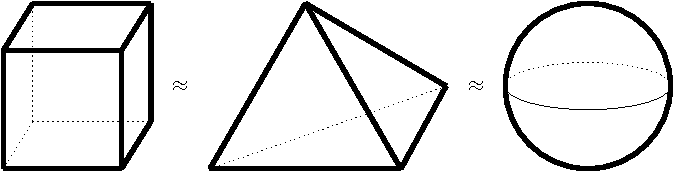
\includegraphics[width=1\linewidth]{H4.pdf}
		\caption{\small\textit{\color{duongvaotoanhoc}Hình $4$: Hình hộp và tứ điện đồng phôi với mặt cầu.}}
		\vspace*{-10pt}
	\end{figure}
	Một ví dụ khác: đĩa mở đơn vị $\mathbb{D} = \{(x,y) \in \mathbb{R}^2: x^2 + y^2 < 1\}$ đồng phôi với toàn bộ mặt phẳng $\mathbb{R}^2$ (mặt dù $\mathbb{D}$ có vẻ ``hữu hạn'' còn $\mathbb{R}^2$ thì vô hạn). Thật vậy, ánh xạ
	\begin{align*}
		f\!:\! \mathbb{D} \!\to\! \mathbb{R}^2,  f(x,y) \!=\! \left(\!\!\frac{x}{1 \!-\! x^2 \!-\! y^2}, \frac{y}{1 \!-\! x^2 \!-\! y^2}\!\right)
	\end{align*}
	là một song ánh liên tục có ánh xạ ngược liên tục $f^{-1}: \mathbb{R}^2 \to \mathbb{D}$ cho bởi công thức
	\begin{align*}
		&f^{-1}(x,y) \\
		= &\left(\!\frac{2x}{\sqrt{4x^2 \!+\! 4y^2 \!+\! 1} \!+\! 1}, \frac{2y}{\sqrt{4x^2 \!+\! 4y^2 \!+\! 1} \!+\! 1}\!\right).
	\end{align*}
	Tương tự, đoạn mở $(0,1)$ đồng phôi với đưởng thẳng thực $\mathbb{R}$ (ta có thể xét $f(x) = \frac{2x-1}{x - x^2}$).
	\vskip 0.1cm
	Ta kết thúc mục này với ví dụ về sự đồng phôi, mà nhìn qua thì có vẻ không tầm thường, của $3$ không gian sau đây (xem Hình $5$).
	\vskip 0.1cm
	$\bullet$ {\it Đĩa thủng} $\mathbb{D}^\ast = \mathbb{D} \setminus \{(0,0)\}$, hình tròn đơn vị (không kể biên) bỏ tâm.
	\vskip 0.1cm
	$\bullet$ {\it Hình vành khăn} $A = \{(x,y) \in \mathbb{R}^2: 1 < x^2 + y^2 < 4\}$, phần mặt phẳng nằm giữa (không kể biên) các đường tròn với tâm $(0,0)$ và bán kính lần lượt là $1$ và $2$.
	\vskip 0.1cm
	$\bullet$ {\it Mặt trụ} $C = \{(x,y,z) \in \mathbb{R}^3: x^2 + y^2 = 1\}$. 
	\begin{figure}[H]
		\vspace*{-5pt}
		\centering\captionsetup{labelformat=empty, justification=centering}
		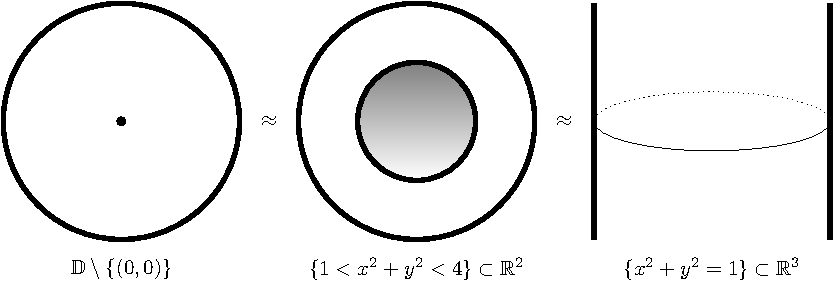
\includegraphics[width=1\linewidth]{H5.pdf}
		\caption{\small\textit{\color{duongvaotoanhoc}Hình $5$: Đĩa thủng, hình vành khăn và mặt trụ đồng phôi với nhau.}}
		\vspace*{-10pt}
	\end{figure}
	Thật vậy, ta có các phép đồng phôi
	\begin{align*}
		&f: \mathbb{D}^\ast \to A,\\
		&f(x,y) \!=\! \left(\!\!\left(\!\!\sqrt{x^2 \!+\! y^2} \!+\! 1\!\!\right)\!x,\left(\!\!\sqrt{x^2 \!+\! y^2} \!+\! 1\!\right)y\!\right)
	\end{align*}
	và
	\begin{align*}
		g\!:\! A \!\to\! C,\,\,\,g(x,y)& = \left(\!\!\frac{x}{\sqrt{x^2 + y^2}},\frac{y}{\sqrt{x^2 + y^2}},\right.\\
		&\left.\frac{x^2\!+\!y^2\!-\!2}{(x^2\!+\!y^2\!-\!1)(4\!-\!x^2\!-\!y^2)}\!\!\right)\!.
	\end{align*}
	$\pmb{2.}$ \textbf{\color{duongvaotoanhoc}Tam giác phân. Định nghĩa mặt}
	\vskip 0.1cm
	Để phát biểu định lý chính của ghi chú này, một thao tác cần thiết là định nghĩa khái niệm mặt (cong). Thực ra đây là một công việc rất khó. Về mặt trực giác, một mặt là một đối tượng hình học mà khi nhìn vào địa phương thì trông nó như mặt phẳng $\mathbb{R}^2$ (hoặc như một đĩa mở, vì ta đã biết rằng $\mathbb{D} \approx \mathbb{R}^2$). Chẳng hạn, bề mặt Trái Đất trông như một mặt phẳng khi nhìn vào lân cận của từng điểm (xem Hình $6$).
	\begin{figure}[H]
		\vspace*{-5pt}
		\centering\captionsetup{labelformat=empty, justification=centering}
		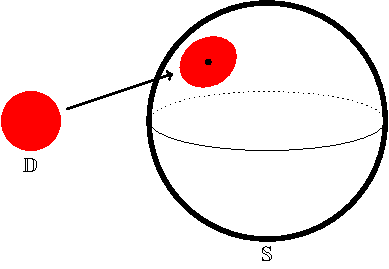
\includegraphics[width=0.7\linewidth]{H6.pdf}
		\caption{\small\textit{\color{duongvaotoanhoc}Hình $6$: Mỗi điểm của mặt cầu đều có một lân cận đồng phôi với $\mathbb{D}$.}}
		\vspace*{-10pt}
	\end{figure}
	Ta sẽ dùng trực giác trên như một định nghĩa không chính thức cho mặt. Về mặt toán học, chúng ta sẽ cần thêm một điều kiện kỹ thuật nữa, và thực ra điều kiện này sẽ giúp chúng ta làm việc được với chứng minh của định lý chính.
	\vskip 0.1cm
	Ta xét tập hợp $\Delta = \{(x,y) \in \mathbb{R}^2: x,y \ge 0, x+y \le 1\}$. Đó là một tam giác trong mặt phẳng, với ba đỉnh lần lượt là $(0,0)$, $(0,1)$ và $(1,0)$. Nó có ba cạnh là ba đoạn thẳng, chúng đồng phôi với đoạn đóng $[0,1]$. Ta gọi $\Delta$ là {\it tam giác tiêu chuẩn}. Một {\it tam giác cong} trên một không gian tôpô $X$ là một phép đồng phôi $\tau: \Delta \to T$, trong đó $\Delta$ là tam giác tiêu chuẩn và $T \subset X$ là một tập con. Ta nhấn mạnh rằng một tam giác cong trên $X$ không chỉ gồm một tập gian con $T$ của $X$ đồng phôi với $\Delta$, mà gồm cả một phép đồng phôi cụ thể $\tau: \Delta \to T$. Điều này cho phép ta nói về $3$ đỉnh và $3$ cạnh của tam giác cong, đó là ảnh của các đỉnh và các cạnh của $\Delta$ bởi $\tau$. Tuy nhiên, nếu không có gì nhầm lẫn, ta sẽ ngầm hiểu rằng tập con $T$ (cùng các đỉnh, các cạnh tương ứng) là một tam giác cong. 
	\vskip 0.1cm
	Một {\it phép tam giác phân} trên $X$ là một họ (có thể vô hạn) $\mathscr{T}$ các tam giác cong trên $X$ sao cho
	\vskip 0.1cm
	$\bullet$ $X = \bigcup_{T \in \mathscr{T}} T$ (họ $\mathscr{T}$ {\it phủ} $X$);
	\vskip 0.1cm
	$\bullet$ nếu $T,T' \in \mathscr{T}$ là hai tam giác phân biệt thì giao $T \cap T'$ hoặc bằng $\varnothing$, hoặc là một đỉnh chung của $T$ và $T'$, hoặc là một cạnh chung của $T$ và $T'$.
	\vskip 0.1cm
	Như vậy, một phép tam giác phân của $X$ là một cách biến dạng liên tục các phiên bản của tam giác chuẩn và dán chúng lại dọc theo các cạnh hoặc các đỉnh để thu được $X$. Dễ thấy một phép đồng phôi sẽ biến một phép tam giác phân của không gian này thành một phép tam phân của không gian kia. Ta có thể dễ dàng tam giác phân bất kỳ đa diện lồi nào. Chẳng hạn, tứ diện có thể được tam giác phân bởi $4$ mặt của nó (là các tam giác). Với hình hộp, ta có thể tam giác phân nó bởi $12$ tam giác, bằng cách chia đôi từng mặt (là các hình chữ nhật) theo một trong hai đường chéo. Đĩa đóng đơn vị $\overline{\mathbb{D}}$ đồng phôi với $\Delta$, ta có thể tam giác phân nó bởi một tam giác cong như trong Hình $7$.
	\begin{figure}[H]
		\vspace*{-5pt}
		\centering\captionsetup{labelformat=empty, justification=centering}
		\includegraphics[width=1\linewidth]{H7.pdf}
		\caption{\small\textit{\color{duongvaotoanhoc}Hình $7$: Tam giác phân đĩa đóng bởi 1 tam giác cong.}}
		\vspace*{-10pt}
	\end{figure}
	Mặt cầu đơn vị $\mathbb{S}$ trong không gian $\mathbb{R}^3$ được xây dựng bằng cách dán hai bán cầu dọc theo đường xích đạo. Dễ thấy mỗi bán cầu này đồng phôi với đĩa đóng đơn vị $\overline{\mathbb{D}}$, trong đó đường xích đạo ứng với đường tròn biên của đĩa. Từ đó ta có thể tam giác phân $\mathbb{S}$ bằng cách dán $2$ bản sao đồng phôi của $\Delta$ như trong Hình $8$ dọc theo đúng các cạnh $xy$, $yz$ và $xz$.
	\begin{figure}[H]
		\vspace*{-5pt}
		\centering\captionsetup{labelformat=empty, justification=centering}
		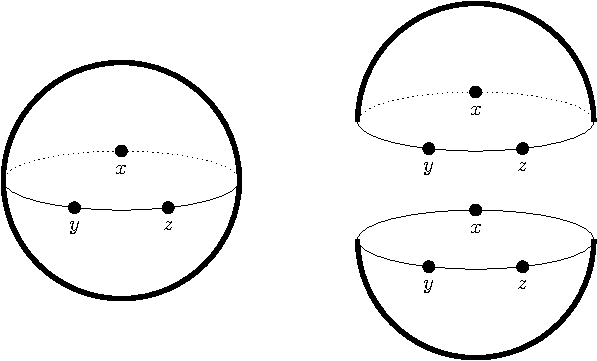
\includegraphics[width=1\linewidth]{H8.pdf}
		\caption{\small\textit{\color{duongvaotoanhoc}Hình $8$: Tam giác phân mặt cầu bởi $2$ tam giác cong.}}
		\vspace*{-5pt}
	\end{figure}
	Mặt phẳng $\mathbb{R}^2$ có thể được tam giác phân bởi một dãy vô hạn các tam giác cong như trong Hình $9$.
	\begin{figure}[H]
		\vspace*{-5pt}
		\centering\captionsetup{labelformat=empty, justification=centering}
		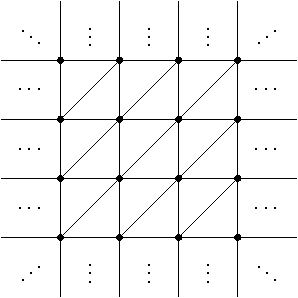
\includegraphics[width=0.7\linewidth]{H9.pdf}
		\caption{\small\textit{\color{duongvaotoanhoc}Hình $9$: Tam giác phân mặt phẳng bởi một dãy vô hạn các tam giác cong.}}
		\vspace*{-10pt}
	\end{figure}
	Chú ý rằng theo định nghĩa của tam giác phân, các cách dán như trong Hình $10$ đều bị cấm (phần màu tím chỉ giao của hai tam giác cong).
	\begin{figure}[H]
		\vspace*{-5pt}
		\centering\captionsetup{labelformat=empty, justification=centering}
		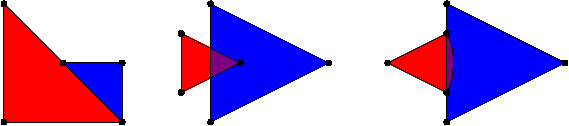
\includegraphics[width=1\linewidth]{H10.pdf}
		\caption{\small\textit{\color{duongvaotoanhoc}Hình $10$: Không phải các phép tam giác phân.}}
		\vspace*{-10pt}
	\end{figure}
	Sau đây là định nghĩa quan trọng nhất của toàn bộ bài viết. Một {\it mặt} là một không gian tôpô $X$ sao cho
	\vskip 0.1cm
	$\bullet$ mỗi điểm $x \in X$ đều có một lân cận đồng phôi với đĩa đóng đơn vị $\overline{\mathbb{D}}$;
	\vskip 0.1cm
	$\bullet$ $X$ {\it liên thông}, nghĩa là với mọi $x, y \in X$, tồn tại một ánh xạ liên tục $\gamma: [0,1] \to X$ sao cho $\gamma(0) = x$ và $\gamma(1) = y$ (ta gọi $\gamma$ là một {\it đường} trên $X$ với điểm đầu $x$ và điểm cuối $y$);
	\vskip 0.1cm
	$\bullet$ $X$ thừa nhận ít nhất một tam giác phân bởi một dãy (hữu hạn hoặc vô hạn) các tam giác cong $T_1,T_2,T_3,\ldots$
	\vskip 0.1cm
	Tính liên thông trong định nghĩa trên cũng có thể phát biểu lại như sau: với mọi $x,y \in X$ và mọi tam giác phân $\mathscr{T}$ của $X$, tồn tại một dãy hữu hạn $T_0,\ldots,T_n \in \mathscr{T}$ sao cho $x \in T_0$, $y \in T_n$ và $T_{i-1} \cap T_i \neq \varnothing$ với $1 \le i \le n$. 
	\vskip 0.1cm
	Định nghĩa trên loại bỏ các mặt có {\it điểm kỳ dị}, chẳng hạn như {\it mặt nón}
	\begin{align*}
		C = \{(x,y,z) \in \mathbb{R}^3: z^2 = x^2 + y^2\},
	\end{align*}
	vì điểm $(0,0,0) \in C$ không có lân cận nào trong $C$ đồng phôi với $\overline{\mathbb{D}}$ (xem Hình $11$).
	\begin{figure}[H]
		\vspace*{-5pt}
		\centering\captionsetup{labelformat=empty, justification=centering}
		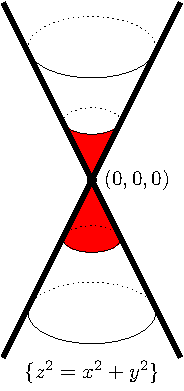
\includegraphics[width=0.35\linewidth]{H11.pdf}
		\caption{\small\textit{\color{duongvaotoanhoc}Hình $11$: $(0,0,0)$ là một điểm kỳ dị của mặt nón.}}
		\vspace*{-10pt}
	\end{figure}
	Nếu mặt $X$ thừa nhận một tam giác phân bởi một số hữu hạn các tam giác cong, ta nói $X$ là một mặt {\it compact}. Ta thấy ngay rằng tứ diện, hình hộp, đĩa đóng $\overline{\mathbb{D}}$ và mặt cầu $\mathbb{S}$ là các mặt compact. Dễ thấy mặt phẳng $\mathbb{R}^2$ không thể được tam giác phân bởi một số hữu hạn các tam giác cong, vì thế $\mathbb{R}^2$ không compact. Mà $\mathbb{D} \approx \mathbb{R}^2$ và tính compact là một bất biến tôpô nên đĩa mở $\mathbb{D}$ cũng không compact.
	\vskip 0.1cm
	$\pmb{3.}$ \textbf{\color{duongvaotoanhoc}Tính đóng và định hướng. Trải phẳng}
	\vskip 0.1cm
	Trong định nghĩa về mặt, ta dùng đĩa đóng $\overline{\mathbb{D}}$ thay cho đĩa mở $\mathbb{D}$. Lí do là vì cách định nghĩa như vậy bao hàm các {\it mặt có biên}, như sau. Cho $X$ là một mặt. Ta nói một điểm $x \in X$ là {\it điểm trong} nếu nó có một lân cận đồng phôi với đĩa mở đơn vị $\overline{\mathbb{D}}$. Ngược lại, ta gọi nó là một {\it điểm biên}. Tập hợp các điểm trong của $X$ được gọi là {\it phần trong} của $X$ và được ký hiệu bởi $X^\circ$. Tập hợp các điểm biên của $X$ được gọi nó là {\it biên} của $X$ và được ký hiệu bởi $\partial X$. 
	\vskip 0.1cm
	Chẳng hạn, ở Hình $1$, ta thấy rằng $\partial \overline{\mathbb{D}}$ là đường tròn đơn vị và $\overline{\mathbb{D}}^\circ = \mathbb{D}$. Trong khi đó, hình hộp, hình cầu, mặt trụ... đều là các mặt không có biên (mọi điểm của chúng đều là điểm trong). Dễ thấy biên và phần trong là các khái niệm tôpô, tức là nếu $f: X \to Y$ là một phép đồng phôi thì $f(\partial X) = \partial Y$ và $f(X^\circ) = Y^\circ$.
	\vskip 0.1cm
	Xét $\mathscr{T}$ là phép một tam giác phân trên một mặt $X$. Giả sử $x$ là một điểm nằm trên một cạnh $a$ của một tam giác cong $T \in \mathscr{T}$, nhưng không phải một đỉnh của $T$. Giao của mọi lân cận của $x$ với $T$ chứa một tập con $D \approx \overline{\mathbb{D}}$, và $x \in \partial D$. Mặt khác, theo định nghĩa tam giác phân, nếu $T' \in \mathscr{T}$ là một tam giác cong khác chứa $x$ thì $a$ là một cạnh của $T'$, nên điều tương tự cũng đúng với giao của mọi lân cận của $x$ với $T'$. Từ đây ta thấy rằng nếu $a$ là một cạnh của ít nhất $3$ tam giác cong thuộc $\mathscr{T}$ thì $x$ không có bất kỳ lân cận nào đồng phôi với $\overline{\mathbb{D}}$. 
	\vskip 0.1cm
	$\bullet$ Nếu $a$ là cạnh của $1$ tam giác cong duy nhất $T \in \mathscr{T}$ thì $x$ không có lân cận nào đồng phôi với $\mathbb{D}$, nên $x \in \partial X$. Trong trường hợp này, mọi điểm của $a$ trừ hai đầu mút đều nằm trên $\partial X$. Hai đầu mút của $a$ cũng nằm trên $\partial X$, vì nếu có một đầu mút $e \in X^\circ$ thì theo định nghĩa, mọi điểm thuộc lân cận đủ nhỏ của $e$ (nói riêng, các điểm nằm trên $a$ đủ gần $e$) cũng phải thuộc $X^\circ$, mâu thuẫn. Vậy $a \subset \partial X$.
	\vskip 0.1cm	
	$\bullet$ Nếu $a$ là cạnh chung của $2$ tam giác cong phân biệt $T,T' \in \mathscr{T}$ thì $x$ có một lân cận $D \approx \overline{\mathbb{D}}$, và $x \in D^\circ \approx \mathbb{D}$, suy ra $x \in X^\circ$.
	\vskip 0.1cm
	Tóm lại, khi ta có một tam giác phân $\mathscr{T}$ của một mặt $X$, mỗi cạnh của một tam giác cong đều nằm trong không quá $2$ tam giác cong, và biên $\partial X$ chính là hợp của tất cả các cạnh chỉ nằm trong đúng $1$ tam giác cong.
	\vskip 0.1cm
	Quay lại với định nghĩa của mặt, ta có thể hiểu rằng một mặt $X$ là compact nếu nó ``chứa mọi điểm biên có thể của nó'', hay chính xác hơn, nếu $Y$ là một mặt chứa $X$ và có cùng phần trong $Y^\circ = X^\circ$ thì ta phải có $Y = X$ (ta có thể đối chiếu với trường hợp đĩa mở $\mathbb{D}$ để hiểu trực giác này hơn). Định lý chính của chúng ta quan tâm đến các mặt {\it đóng}, tức là compact và không có biên. Hiển nhiên tính đóng là một bất biến tôpô. Chẳng hạn, mặt cầu $\mathbb{S}$ là một mặt đóng, trong khi đĩa đóng $\overline{\mathbb{D}}$ và đĩa mở $\mathbb{D}$ đều không phải các mặt đóng.
	\vskip 0.1cm
	Sau đây là một ví dụ quan trọng, là một phần trong phát biểu của định lý chính. Ta gọi {\it mặt xuyến} là mặt tròn xoay $\mathbb{T}$ thu được khi xoay một đường tròn với bán kính $r$ trong mặt phẳng $x=a$ của $\mathbb{R}^3$, với $a > r$, quanh trục $Oz$ (ta sẽ không đưa ra phương trình cụ thể cho $\mathbb{T}$ mặt dù ta có thể làm điều đó). Đó chính là bề mặt của chiếc phao. Ta có thể thu được $\mathbb{T}$ từ $\overline{\mathbb{D}}$ như sau. Ta biết rằng $\overline{\mathbb{D}}$ đồng phôi với hình vuông đặc (gồm cả phần trong và biên). Ta ``dán cùng chiều'' cặp cạnh đối của hình vuông này (nghĩa là ta đồng nhất các cặp điểm tương ứng trên $2$ cạnh) để thu được mặt trụ compact $C$ - đây là một mặt với biên gồm $2$ đường tròn rời nhau ($2$ đường tròn này là cặp cạnh đối còn lại của hình vuông sau khi dán hai đầu mút). Cuối cùng, ta dán cùng chiều $2$ đường tròn biên của $C$ để thu được mặt xuyến $\mathbb{T}$. Đây là một mặt không có biên. 
	\begin{figure}[H]
		\vspace*{-5pt}
		\centering\captionsetup{labelformat=empty, justification=centering}
		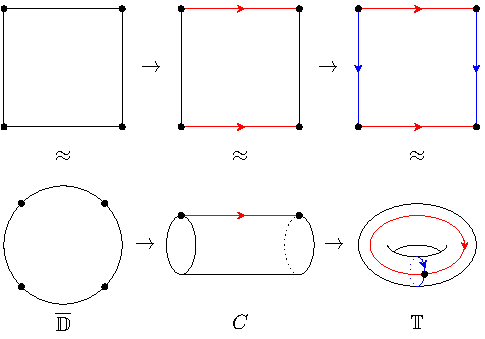
\includegraphics[width=1\linewidth]{H12.pdf}
		\caption{\small\textit{\color{duongvaotoanhoc}Hình $12$: Xây dựng mặt xuyến $\mathbb{T}$ bằng cách dán các cặp cạnh đối của hình vuông.}}
		\vspace*{-10pt}
	\end{figure}
	Trong Hình $12$, ta thể hiện chiều khi dán các cặp cạnh đối bằng các mũi tên. Chú ý rằng $4$ đỉnh của hình vuông sau cùng chỉ còn là $1$ điểm trên $\mathbb{T}$. Đây là một {\it trải phẳng} của $\mathbb{T}$, thứ ta sẽ nói rõ hơn ở dưới. Một tam giác phân của $\mathbb{T}$ có thể được cho bởi Hình $13$ (khi đếm số đỉnh và số cạnh, chú ý đến các cạnh đã được dán lại với nhau). Nói riêng, $\mathbb{T}$ compact, vì thế đóng.
	\begin{figure}[H]
		\vspace*{-5pt}
		\centering\captionsetup{labelformat=empty, justification=centering}
		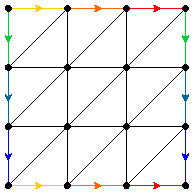
\includegraphics[width=0.7\linewidth]{H13.pdf}
		\caption{\small\textit{\color{duongvaotoanhoc}Hình $13$: Tam giác phân mặt xuyến bằng $9$ đỉnh, $27$ cạnh và $18$ tam giác cong.}}
		\vspace*{-10pt}
	\end{figure}
	Tổng quát hơn, cho $X$ là một mặt compact tùy ý và $\mathscr{T}$ là một tam giác phân của $X$. Ta đặt tất cả các tam giác cong của $\mathscr{T}$ (kể cả biên) vào các vị trí rời nhau trên mặt phẳng. Sau đó, ta lần lượt dán các tam giác cong có ít nhất một cặp cạnh chung theo đúng chiều của cặp cạnh chung đó, rồi xóa cặp cạnh chung đó đi. Sau một số hữu hạn thao tác như vậy, do tính compact và tính liên thông của $X$, ta thu được một ``đa giác'' mà ở đó một số cặp cạnh được đồng nhất với nhau theo chiều nào đó (chẳng hạn, sau khi dán tất cả các cặp cạnh có thể từ tam giác phân ở Hình $13$ để thu được Hình $12$, ta còn lại một ``tứ giác'' trong đó các cặp cạnh đối được đồng nhất với nhau). Đó là một {\it trải phẳng} của mặt $X$. Chú ý rằng có nhiều thứ tự thực hiện phép dán các cặp cạnh chung, nên một mặt có thể có những trải phẳng khác nhau. Chú ý thêm rằng hoàn toàn có thể có những cạnh chỉ xuất hiện một lần, những cạnh này tạo thành biên của mặt $X$. Nói riêng, nếu mặt $X$ đóng (không có biên) thì đa giác sau cùng thu được có số cạnh chẵn. 
	\vskip 0.1cm
	Chẳng hạn, từ phép tam giác phân bởi $2$ tam giác cong, ta thu được trải phẳng của mặt cầu $\mathbb{S}$ như ở Hình $14$, bằng cách dán $2$ cặp cạnh kề của hình vuông.
	\begin{figure}[H]
%		\vspace*{-5pt}
		\centering\captionsetup{labelformat=empty, justification=centering}
		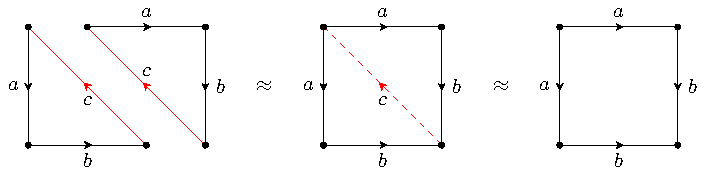
\includegraphics[width=1\linewidth]{H14.pdf}
		\caption{\small\textit{\color{duongvaotoanhoc}Hình $14$: Trải phẳng của mặt cầu.}}
		\vspace*{-10pt}
	\end{figure}
	Tiếp theo, ta nói về định hướng. Đây là một khái niệm tương đối khó định nghĩa chặt chẽ (ngay cả định nghĩa cho mặt phẳng cũng cần đến đại số tuyến tính). Chúng ta sẽ chỉ đưa ra một định nghĩa trực giác như sau. Một mặt $X$ được gọi là {\it hai phía} hay {\it khả định hướng} nếu với mọi điểm $x \in X^\circ$ và mọi đường $\gamma \subset X^\circ$ xuất phát và kết thúc tại $x$, nếu ta đi dọc theo $\gamma$ thì ta vẫn ở cùng phía của mặt như khi bắt đầu. Ngược lại, ta nói $X$ là {\it một phía} hay {\it bất khả định hướng}.
	\vskip 0.1cm
	Nói cách khác, mặt $X$ là một phía nếu ta có thể đi từ phía này sang phía kia của một điểm trong mà không cần đi qua biên của mặt. Tính một/hai phía là một bất biến tôpô, một mặt một phía không thể đồng phôi với một mặt hai phía. Các mặt đã giới thiệu như đĩa đóng, đĩa mở, mặt cầu, mặt trụ, mặt xuyến... đều là các mặt hai phía. Ví dụ đầu tiên và rất nổi tiếng về mặt một phía là {\it băng M\"obius} $\mathbb{M}$, mặt thu được khi dán ngược chiều một cặp cạnh đối của một hình vuông. Mặt này có thể được ``nhúng'' vào $\mathbb{R}^3$ như trong Hình $15$.
	\begin{figure}[H]
		\vspace*{-5pt}
		\centering\captionsetup{labelformat=empty, justification=centering}
		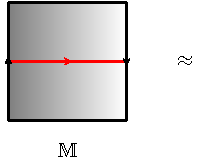
\includegraphics[width=0.48\linewidth]{H15_1.pdf}
		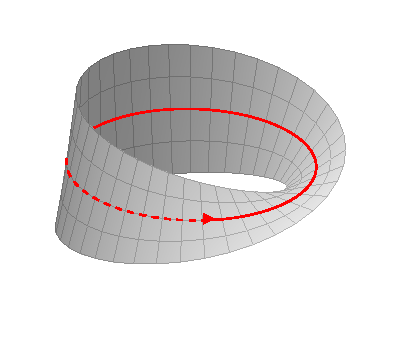
\includegraphics[width=0.48\linewidth]{H15_2.pdf}
		\caption{\small\textit{\color{duongvaotoanhoc}Hình $15$: Băng M\"obius khi trải phẳng và khi được đặt trong không gian $3$--chiều.}}
		\vspace*{-10pt}
	\end{figure}
	Để thấy tại sao $\mathbb{M}$ là một phía, hãy hình dung một con bọ nằm trên một điểm trong của $\mathbb{M}$. Con bọ có thể đi từ phía này sang phía kia của băng M\"obius mà không đi qua biên.
	\vskip 0.1cm
	Tổng quát hơn, bất cứ mặt nào chứa một tập con đồng phôi với $\mathbb{M}$ đều là mặt một phía. Sau đây là các ví dụ khác về các mặt đóng (không có biên) và một phía. Chúng được xây dựng bằng cách dán cách cặp cạnh đối của hình vuông tương tự như mặt xuyến (xem Hình $12$), nhưng theo các chiều khác nhau. {\it Chai Klein} $\mathbb{K}$ thu được từ hình vuông bằng cách dán cùng chiều một cặp cạnh của hình vuông, và dán ngược chiều cặp cạnh còn lại. Trong khi đó, {\it mặt phẳng xạ ảnh} $\mathbb{P}$ thu được từ hình vuông bằng cách dán ngược chiều các cặp cạnh của hình vuông. Trải phẳng của $\mathbb{K}$ và $\mathbb{P}$ được cho bởi Hình $16$. Không giống như mặt xuyến và băng M\"obius, hai mặt vừa xây dựng đều không phải là các thực thể có ở ngoài đời thực (chúng không ``nhúng'' được vào $\mathbb{R}^3$).
	\begin{figure}[H]
		\vspace*{-5pt}
		\centering\captionsetup{labelformat=empty, justification=centering}
		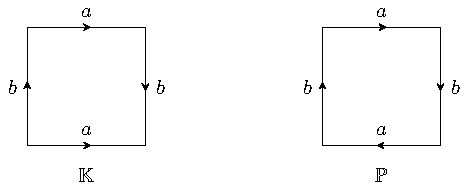
\includegraphics[width=1\linewidth]{H16.pdf}
		\caption{\small\textit{\color{duongvaotoanhoc}Hình $16$: Trải phẳng của chai Klein và mặt phẳng xạ ảnh.}}
		\vspace*{-10pt}
	\end{figure}
	Các mặt $\mathbb{K}$ và $\mathbb{P}$ đều là mặt một phía, ví chúng chứa một tập con đồng phôi với $\mathbb{M}$ (xem Hình $17$).
	\begin{figure}[H]
		\vspace*{-5pt}
		\centering\captionsetup{labelformat=empty, justification=centering}
		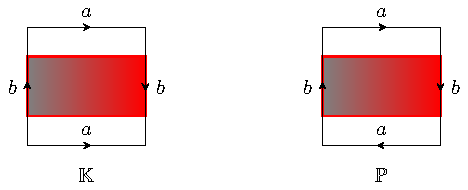
\includegraphics[width=1\linewidth]{H17.pdf}
		\caption{\small\textit{\color{duongvaotoanhoc}Hình $17$: Chai Klein và mặt phẳng xạ ảnh đều chứa băng M\"obius.}}
		\vspace*{-10pt}
	\end{figure}
	Như đã thấy ở các ví dụ trên, trải phẳng là một công cụ đắc lực để mô tả các mặt. Chúng ta sẽ sớm thấy rằng nó đóng vai trò quan trọng trong chứng minh của định lý chính. Trước khi kết thúc mục này, nhận xét rằng ta có thể xây dựng một mặt tùy ý bằng cách dán (cùng chiều hoặc ngược chiều) một số cặp cạnh của một ``đa giác cong'' (không tự cắt, hay còn gọi là {\it đơn}) trên mặt phẳng. Đa giác cong ở đây có thể có số cạnh bằng $2$, khác với khái niệm đa giác lồi theo nghĩa cổ điển (ít nhất phải có $3$ cạnh). Điều này cho phép ta thu được hai trải phẳng đơn giản hơn của mặt cầu $\mathbb{S}$ và mặt phẳng xạ ảnh $\mathbb{P}$ như trong Hình $18$.
	\begin{figure}[H]
		\vspace*{-5pt}
		\centering\captionsetup{labelformat=empty, justification=centering}
		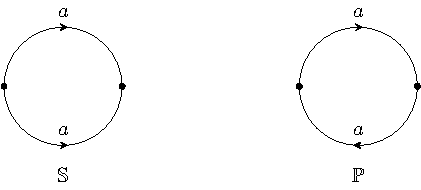
\includegraphics[width=1\linewidth]{H18.pdf}
		\caption{\small\textit{\color{duongvaotoanhoc}Hình $18$: Trải phẳng của mặt cầu và mặt phẳng xạ ảnh bằng ``nhị giác''.}}
		\vspace*{-10pt}
	\end{figure}
	$\pmb{4.}$ \textbf{\color{duongvaotoanhoc}Tổng liên thông. Phát biểu định lý}
	\vskip 0.1cm
	Khi đã định nghĩa các mặt đóng cơ bản: mặt cầu $\mathbb{S}$, mặt xuyến $\mathbb{T}$, mặt phẳng xạ ảnh $\mathbb{P}$... ta có thể xây dựng thêm các mặt mới từ chúng bằng phép toán sau đây. 
	\vskip 0.1cm
	Cho $X$ và $Y$ là hai mặt. Ta xét hai đĩa đóng $\overline{\mathbb{D}} \approx D_1 \subset X^\circ$ và $\overline{\mathbb{D}} \approx D_2 \subset Y^\circ$. Khi đó, $X \setminus D_1^\circ$, $Y \setminus D_2^\circ$ là các mặt có biên lần lượt là $\partial X \sqcup \partial D_1$ và $\partial Y \sqcup \partial D_2$ (ở đây, ta dùng ký hiệu $\sqcup$ -- {\it hợp rời} -- để nhấn mặt rằng đó là hợp của hai tập hợp rời nhau). Ta dán hai mặt có biên này dọc theo hai đường tròn $\partial D_1$ và $\partial D_2$ với nhau. Điều thú vị nhất là cách xây dựng này không phụ thuộc vào cách chọn các đĩa $D_1,D_2$ và cách dán $\partial D_1$ với $\partial D_2$ (nghĩa là với việc hai cách lựa chọn các dữ liệu này khác nhau, ta thu được hai mặt đồng phôi). Ta bỏ qua chứng minh của tính chất này vì tính kỹ thuật của nó. Mặt thu được (sai khác đồng phôi) là một mặt được ký hiệu bởi $X \# Y$ và được gọi là {\it tổng liên thông} của $X$ và $Y$.
	\vskip 0.1cm
	Giả sử $\mathscr{T}$ và $\mathscr{T}'$ lần lượt là các tam giác phân của $X$ và $Y$ sao cho có ít nhất một tam giác cong $T \in \mathscr{T}$ nằm trong $X^\circ$ và ít nhất một tam giác cong $T' \in \mathscr{T}'$ nằm trong $Y^\circ$ (ta luôn có thể giả sử sự tồn tại của một tam giác phân như vậy: nếu $T$ chưa nằm trong $X$, ta tiếp tục tam tam giác phân bản thân $T$ sao cho ít nhất một trong các giác cong thu được nằm trong $T^\circ$ -- vì thế cũng nằm trong $X^\circ$; và tương tự cho $T'$). Khi đó, ta có thể dễ dàng xây dựng một phép tam giác phân của $X \# Y$ bằng cách dán $X \setminus T^\circ$ với $X \setminus T'^\circ$ dọc theo từng cạnh $T$ với từng cạnh của $T'$ (nhắc lại rằng $T \approx T' \approx \Delta \approx \overline{\mathbb{D}}$). Nói riêng, nếu $X$ và $Y$ compact thì $X \# Y$ cũng compact. Ngoài ra, biên của $X \# Y$ là $\partial(X \# Y) = \partial X \sqcup \partial Y$. Vì thế, nếu $X$ và $Y$ là các mặt đóng thì $X \# Y$ cũng vậy.  
	\vskip 0.1cm
	Một tính chất nữa chúng ta nhắc đến (mà không chứng minh) là:
	\begin{center}
		{\it Tổng liên thông của hai mặt hai phía lại là một mặt hai phía. Tổng liên thông của một mặt một phía với một mặt hai phía là một mặt một phía.}
	\end{center}
	Tuy nhiên, tổng liên thông của hai mặt một phía vẫn có thể là một mặt một phía. Chẳng hạn, Hình $19$ cho thấy rằng $\mathbb{P} \# \mathbb{P} \approx \mathbb{K}$ (chú ý rằng ta đã thực hiện hai tao tác trên trải phẳng là {\it cắt đa giác để tạo ra một cặp cạnh mới} và {\it dán dọc theo một cặp cạnh khác}). 
	\begin{figure}[H]
		\vspace*{-5pt}
		\centering\captionsetup{labelformat=empty, justification=centering}
		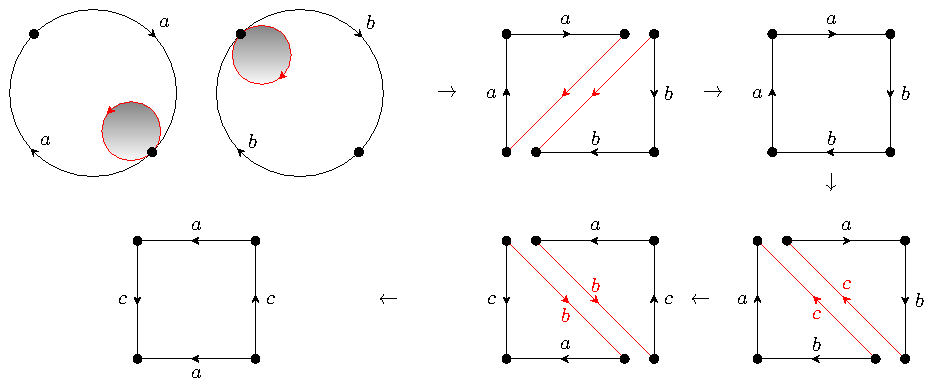
\includegraphics[width=1\linewidth]{H19.pdf}
		\caption{\small\textit{\color{duongvaotoanhoc}Hình $19$: Tổng liên thông của hai mặt phẳng xạ ảnh là (chính xác hơn, đồng phôi với) chai Klein.}}
		\vspace*{-10pt}
	\end{figure}
	Tổng liên thông có tính giao hoán (sai khác đồng phôi), $X \# Y \approx Y \# X$, cũng như tính kết hợp, $(X \# Y) \# Z \approx X \# (Y \# Z)$. Chúng cho phép ta định nghĩa tổng liên thông của một số hữu hạn bất kỳ các mặt. Với $g$ là số nguyên dương, ta sẽ ký hiệu tổng liên thông của $g$ mặt (đồng phôi với) $X$ bởi $X^{\# g}$. Mặt cầu $\mathbb{S}$ đóng vai trò như phần tử trung lập của tổng liên thông (vì thế, ta quy ước $X^{\# 0} := \mathbb{S}$). Thật vậy, xét một mặt $X$ tùy ý và một đĩa $\overline{\mathbb{D}} \approx D \subset X^\circ$. Xét tam giác phân ở Hình $8$, nghĩa là $\mathbb{S} = U \cup V$, trong đó $U \approx V \approx \overline{\mathbb{D}}$ là hai bán cầu (đóng), và $U \cap V = \partial U = \partial V$ là một đường tròn (đường xích đạo). Rõ ràng, khi dán $X \setminus D^\circ$ với $\mathbb{S} \setminus U^\circ = V$ dọc theo $\partial D \approx \partial V$, ta thu được một mặt đồng phôi với $X$, vì $V^\circ \approx \mathbb{D} \approx D^\circ$. Vậy $X \# \mathbb{S} \approx X$.
	\vskip 0.1cm
	Một họ các mặt mới mà ta thu được bằng phép toán ``$\#$'' là ``mặt xuyến với $g$ quai cầm'' $\mathbb{T}^{\# g}$, với $g \ge 1$. Chẳng hạn, tổng liên thông $\mathbb{T}^{\#2} \approx \mathbb{T} \# \mathbb{T}$ được mô tả như trong Hình $20$. Trải phẳng của nó là một bát giác như trong Hình $21$.
	\begin{figure}[H]
		\vspace*{-5pt}
		\centering\captionsetup{labelformat=empty, justification=centering}
		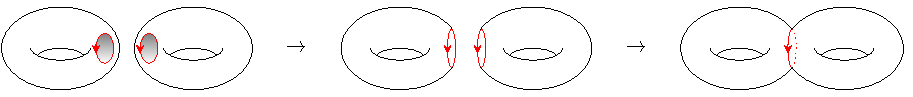
\includegraphics[width=1\linewidth]{H20.pdf}
		\caption{\small\textit{\color{duongvaotoanhoc}Hình $20$: Tổng liên thông của $2$ mặt xuyến trong không gian $3$--chiều.}}
		\vspace*{-10pt}
	\end{figure}
	\begin{figure}[H]
		\vspace*{-5pt}
		\centering\captionsetup{labelformat=empty, justification=centering}
		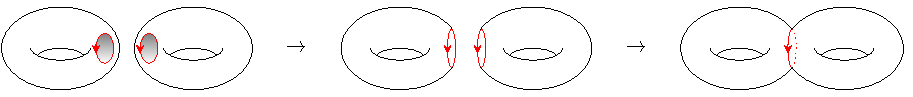
\includegraphics[width=1\linewidth]{H20.pdf}
		\caption{\small\textit{\color{duongvaotoanhoc}Hình $21$: Tổng liên thông của $2$ mặt xuyến được trải phẳng.}}
		\vspace*{-10pt}
	\end{figure}
	Tương tự, mặt  $\mathbb{T}^{\# g}$ có trải phẳng là một $4g$--giác.
	\vskip 0.1cm
	Chúng ta đã sẵn sàng phát biểu định lý chính của bài viết này.
	\vskip 0.1cm
	{\it Mọi mặt đóng đều đồng phôi với duy nhất một trong các mặt sau đây.
	\vskip 0.1cm
	$\bullet$ Mặt cầu $\mathbb{S}$.
	\vskip 0.1cm
	$\bullet$ Tổng liên thông $\mathbb{T}^{\# g}$ của $g$ mặt xuyến, với $g$ là một số nguyên dương.
	\vskip 0.1cm
	$\bullet$ Tổng liên thông $\mathbb{P}^{\# g}$ của $g$ mặt phẳng xạ ảnh, với $g$ là một số nguyên dương.}
	\vskip 0.1cm
	Trước khi bắt đầu chứng minh định lý chính ở mục sau, ta kết thúc mục này bằng ví dụ thú vị sau đây (nó cũng đóng vai trò trong chứng minh của định lý). Hiển nhiên mặt xuyến $\mathbb{T}$ và chai Klein $\mathbb{K}$ không đồng phôi, tuy nhiên, ta sẽ chỉ ra rằng $\mathbb{P} \# \mathbb{T} \approx \mathbb{P} \# \mathbb{K}$ (nói riêng, ta không có tính chất giản ước cho phép toán ``$\#$'' như đối với phép cộng và phép nhân thông thường). Thật vậy, các tổng liên thông $\mathbb{P} \# \mathbb{T}$ và $\mathbb{P} \# \mathbb{K}$ lần lượt được mô tả ở Hình $22$ và $23$.
	\begin{figure}[H]
		\vspace*{-5pt}
		\centering\captionsetup{labelformat=empty, justification=centering}
		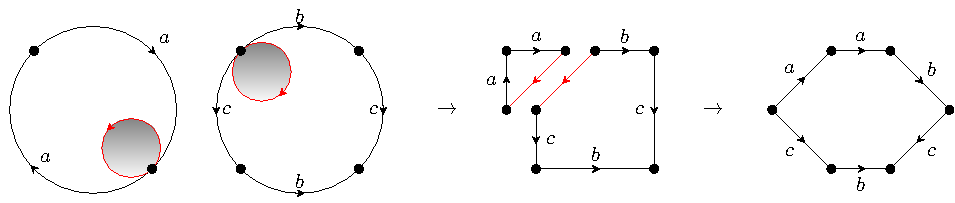
\includegraphics[width=1\linewidth]{H22.pdf}
		\caption{\small\textit{\color{duongvaotoanhoc}Hình $22$: Tổng liên thông của mặt phẳng xạ ảnh và mặt xuyến.}}
		\vspace*{-10pt}
	\end{figure}
	\begin{figure}[H]
		\vspace*{-5pt}
		\centering\captionsetup{labelformat=empty, justification=centering}
		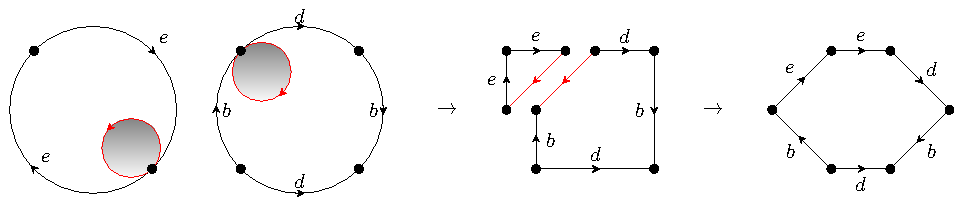
\includegraphics[width=1\linewidth]{H23.pdf}
		\caption{\small\textit{\color{duongvaotoanhoc}Hình $23$: Tổng liên thông của mặt phẳng xạ ảnh và chai Klein.}}
		\vspace*{-10pt}
	\end{figure}
	Tương tự như khi đã chỉ ra rằng $\mathbb{K} \approx \mathbb{P}^{\# 2}$ (xem Hình $19$), bằng cách thực hiện các thao tác cắt dán như trong Hình $24$, ta thấy rằng $\mathbb{P} \# \mathbb{T} \approx \mathbb{P} \# \mathbb{K} \approx \mathbb{P}^{\# 3}$.
	\begin{figure}[H]
		\vspace*{-5pt}
		\centering\captionsetup{labelformat=empty, justification=centering}
		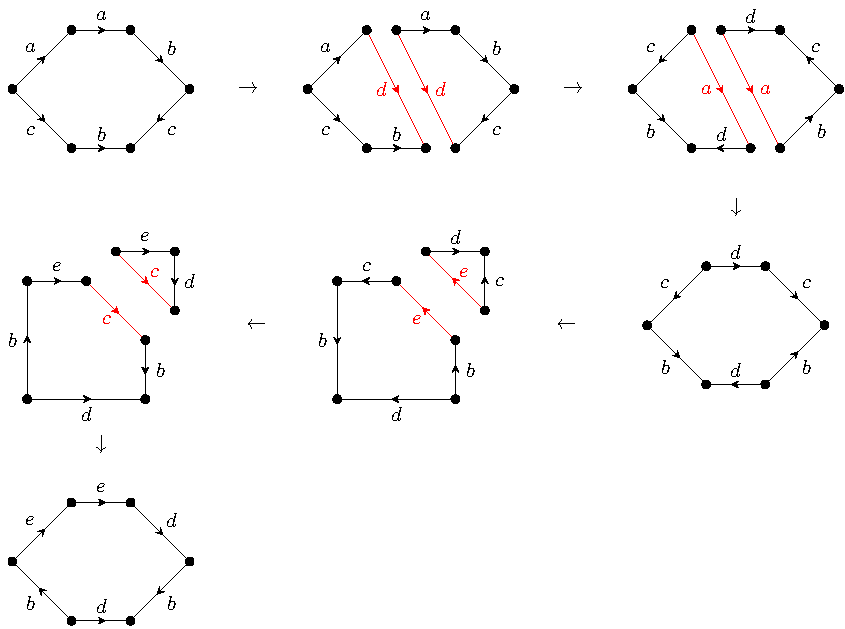
\includegraphics[width=1\linewidth]{H24.pdf}
		\caption{\small\textit{\color{duongvaotoanhoc}Hình $24$: Cắt, rồi dán theo cạnh $a$, rồi lại cắt, cuối cùng dán theo cạnh $c$.}}
		\vspace*{-10pt}
	\end{figure}
	$\pmb{5.}$ \textbf{\color{duongvaotoanhoc}Ký hiệu của mặt đã trải phẳng. Chứng minh định lý}
	\vskip 0.1cm
	Trải phẳng cho phép chúng ta đưa việc phân loại mặt đóng từ một bài toán tôpô thành một bài toán hình học tổ hợp. Để mô tả một mặt compact đã trải phẳng, ta dùng khái niệm sau đây. Cho $X$ là một mặt compact và xét một trải phẳng của $X$. Đó là một đa giác cong hữu hạn với một số cặp cạnh được dán lại với nhau theo một chiều nào đó. Ta dùng các chữ cái để đặt tên cho các cạnh của đa giác cong sao cho các cạnh được dùng một chữ cái khi và chỉ khi chúng được dán lại. Ta đánh mũi tên cho các cạnh để thể hiện chiều dán; đối với những cạnh biên (chỉ xuất hiện một lần, không dán với cạnh nào khác) thì ta đánh mũi tên tùy ý. Ta bắt đầu từ một đỉnh tùy ý và lần lượt đi qua các cạnh của đa giác cong theo một chiều xác định trên mặt phẳng (chẳng hạn, ngược chiều kim đồng hồ) và lần lượt viết tên các cạnh thành một dãy theo quy tắc sau: nếu cạnh $a$ cùng chiều với hướng đi đã chọn thì viết $a$, ngược lại thì viết $a^{-1}$. Ta thu được một dãy ký tự, được gọi là một {\it ký hiệu} của mặt $X$.
	\vskip 0.1cm
	Chẳng hạn, mặt cầu có thể được mô tả bởi ký hiệu $aa^{-1}$ hoặc $abb^{-1}a^{-1}$, mặt xuyến có thể được mô tả bởi ký hiệu $aba^{-1}b^{-1}$, mặt phẳng xạ ảnh có thể được mô tả bởi ký hiệu $aa$ hoặc $abab$, chai Klein có thể được mô tả bởi ký hiệu $aba^{-1}b$ (xem các Hình $12$, $14$, $16$ và $18$).
	\vskip 0.1cm
	Ký hiệu cho phép ta mô tả tổng liên thông một cách đơn giản. Thật vậy, giả sử $X, Y$ là các mặt compact, $S_1$ là một ký hiệu của $X$ và $S_2$ là một ký hiệu của $Y$. Ta khoét một đĩa mở $D_1^\circ$ khỏi $X$ sao cho biên $\partial D_1$ đi qua đỉnh đầu (cũng là đỉnh cuối) của đường đi mà ta đã chọn để định nghĩa $S_1$. Mặt thu được được cho bởi ký hiệu $S_1a$, với $a$ là một chữ cái chưa xuất hiện trong $S_1$ (dùng để ký hiệu $\partial D_1$). Khoét một đĩa mở $D_2^\circ$ khỏi $Y$ theo cách tương tự, ta thu được mặt $S_2$ cho bởi ký hiệu $aS_2$. Dán hai mặt vừa thu được theo cạnh $a$, ta thu được tổng liên thông $X \# Y$, được cho bởi ký hiệu $S_1S_2$. Tóm lại, ta chỉ cần viết một ký hiệu của $X$ liền với một ký hiệu của $Y$ để thu được một ký hiệu của $X \# Y$. Chẳng hạn, mặt $\mathbb{T}^{\# g}$ được mô tả bởi ký hiệu $a_1b_1a_1^{-1}b_1^{-1}a_2b_2a_2^{-1}b_2^{-1}\ldots a_gb_ga_g^{-1} b_g^{-1}$, trong khi mặt $\mathbb{P}^{\# g}$ được mô tả bởi ký hiệu $a_1a_1a_2a_2\ldots a_ga_g$.
	\vskip 0.1cm
	Ta bắt đầu chứng minh một nửa của định lý chính bằng cách chỉ ra rằng mọi mặt đóng đều đồng phôi với một trong các mặt $\mathbb{S}$, $\mathbb{T}^{\#g}$ hoặc $\mathbb{P}^{\#g}$ (với $g \ge 1$). Xét $X$ là một mặt đóng. Ta trải phẳng nó, đặt tên và định hướng các cạnh một cách thích hợp. Lúc này, đa giác cong thu được gồm các cặp cạnh (vì $X$ không có biên). Chứng minh được chia thành $4$ bước như sau.
	\vskip 0.1cm
	{\bf\color{duongvaotoanhoc} Bước $\pmb{1.}$ Khử các cặp cạnh kề dạng $\{a,a^{-1}\}$.} Ta có thể giả sử đa giác cong thu được có ít nhất $4$ cạnh, vì nếu nó chỉ có một cặp cạnh thì $X \approx \mathbb{S}$ hoặc $X \approx \mathbb{P}$, tùy theo cách hai cặp cạnh này được dán với nhau (xem Hình $18$). Giả sử có một cặp cạnh kề dạng $\{a,a^{-1}\}$. Ta có thể dán nó lại để khử nó khỏi phép trải phẳng, như trong Hình $25$.
	\begin{figure}[H]
		\vspace*{-5pt}
		\centering\captionsetup{labelformat=empty, justification=centering}
		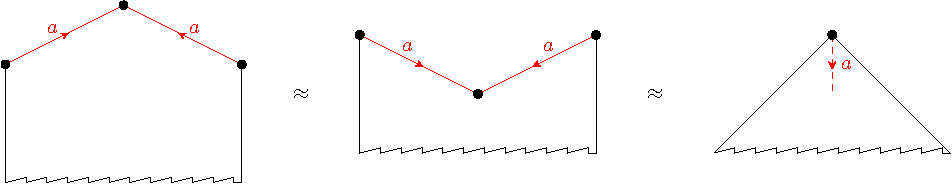
\includegraphics[width=1\linewidth]{H25.pdf}
		\caption{\small\textit{\color{duongvaotoanhoc}Hình $25$: Khử các cặp cạnh kề dạng $\{a,a^{-1}\}$.}}
		\vspace*{-10pt}
	\end{figure}
	Ta lặp lại thao tác khử này cho đến khi $X$ có chỉ còn $2$ cạnh hoặc không còn cặp cạnh kề nào như trên.
	\vskip 0.1cm
	{\bf\color{duongvaotoanhoc} Bước $\pmb{2.}$ Đưa về đa giác cong mà mọi đỉnh đều được dán lại thành một đỉnh.} Đối với mặt xuyến cho bởi ký hiệu $aba^{-1}b^{-1}$, ta thấy rằng $4$ đỉnh của trải phẳng trên được dán lại thành một đỉnh duy nhất. Ta sẽ làm điều này cho mặt đóng $X$ tùy ý. Nếu $x$ là một đỉnh của đa giác cong, ta ký hiệu bởi $[x]$ tập hợp các đỉnh được dán với $x$. Rõ ràng, $[x] = [y]$ nếu $x$ và $y$ được dán với nhau và $[x] \cap [y] = \varnothing$ nếu không.
	\vskip 0.1cm
	Giả sử $x$ và $y$ là hai đỉnh của đa giác cong không được dán với nhau. Ký hiệu bởi $b$ cạnh với hai đầu mút $x,y$, và định hướng lại (nếu cần) sao cho $x$ là điểm cuối của $b$. Ký hiệu bởi $a$ cạnh kề với $b$ tại đầu mút $x$ và gọi $z$ là đầu mút còn lại. Chú ý các cạnh $a$ và $b$ không được dán với nhau (vì nếu vậy thì $x$ phải là điểm cuối của $a$, từ đó ta thu được một cặp cạnh kề nhau dạng $\{a,a^{-1}\}$, mâu thuẫn với giả sử rằng ta đã thực hiện triệt để Bước $1$). Định hướng lại $a$ nếu cần để $x$ là điểm cuối. Ta cắt đa giác cong theo một cạnh $c$ từ $z$ đến $y$, và dán lại dọc theo cạnh $a$. Nếu $[x]$ có ít nhất hai đỉnh thì ở đa giác cong mới thu được, số đỉnh của $[x]$ giảm đi $1$ và số đỉnh của $[y]$ tăng thêm $1$ (xem Hình $26$).
	\begin{figure}[H]
		\vspace*{-5pt}
		\centering\captionsetup{labelformat=empty, justification=centering}
		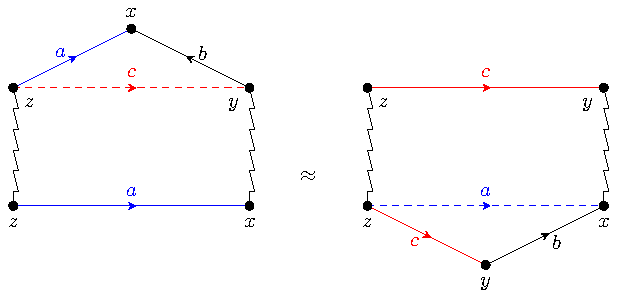
\includegraphics[width=1\linewidth]{H26.pdf}
		\caption{\small\textit{\color{duongvaotoanhoc}Hình $26$: Giảm số đỉnh được dán với $x$ đi 1 và tăng số đỉnh được dán với $y$ thêm $1$.}}
		\vspace*{-10pt}
	\end{figure}
	Ta lặp lại quá trình trên cho đến khi $[x] = \{x\}$. Lúc này, ta thu được một cặp cạnh kề dạng $\{a,a^{-1}\}$ với điểm cuối là $x$ và ta quay lại Bước $1$. Thực hiện phép giản ước ở Bước $1$, ta xóa đỉnh $x$ khỏi đa giác cong, làm giảm tổng số đỉnh (sau khi đã đồng nhất các đỉnh được dán với nhau) đi $1$. Lặp lại toàn bộ quá trình trên (gồm cả Bước $1$ và Bước $2$), sau cùng ta thu được một đa giác cong mà mọi đỉnh đều được dán thành một đỉnh duy nhất.
	\vskip 0.1cm
	{\bf\color{duongvaotoanhoc} Bước $\pmb{3.}$ Thay các cặp cạnh không kề nhau dạng $\{b,b\}$ bởi các cặp cạnh kề nhau.} Giả sử có một cặp cạnh không kề nhau dạng $\{b,b\}$ (dạng $\{b^{-1},b^{-1}\}$ đưa được về dạng này bằng cách định hướng lại). Ta cắt đa giác cong theo một cạnh $a$ nối $2$ điểm cuối của hai cạnh $b$, rồi dán lại dọc theo cạnh $b$ như trong Hình $27$. Chú ý rằng các cặp cạnh kề dạng $\{c,c\}$ hoặc  $\{c^{-1},c^{-1}\}$ (với $c \neq b$) không bị ảnh hưởng bởi thao tác này. Đồng thời, mọi đỉnh vẫn được dán thành một đỉnh duy nhất.
	\begin{figure}[H]
		\vspace*{-5pt}
		\centering\captionsetup{labelformat=empty, justification=centering}
		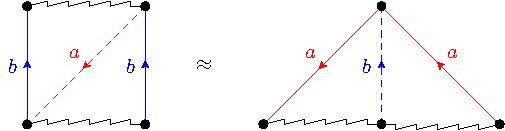
\includegraphics[width=1\linewidth]{H27.pdf}
		\caption{\small\textit{\color{duongvaotoanhoc}Hình $27$: Thay cặp cạnh $\{b,b\}$ bởi cặp cạnh kề nhau $\{a,a\}$.}}
		\vspace*{-10pt}
	\end{figure}
	Lặp lại Bước $3$ cho đến khi mọi cặp cạnh dạng $\{b,b\}$ hoặc $\{b^{-1},b^{-1}\}$ đều kề nhau.
	\vskip 0.1cm
	{\bf\color{duongvaotoanhoc} Bước $\pmb{4.}$ Xử lý các cặp cạnh không kề nhau dạng $\{c,c^{-1}\}$.} Giả sử rằng tồn tại một cặp cạnh không kề nhau dạng $\{c,c^{-1}\}$. Đương nhiên, ta có thể giả sử $c$ là cạnh đầu tiên của đường đi đã chọn, nghĩa là $X$ được cho bởi ký hiệu $cAc^{-1}B$ với $A,B$ là các dãy ký tự khác rỗng. Giả sử phản chứng rằng không có cạnh nào trong $A$ được dán với một cạnh khác trong $B$. Như vậy, các sự dán cạnh chỉ xảy ra trên $A$, trên $B$ hoặc trên cặp $\{c,c^{-1}\}$. Nói riêng, hai đầu mút của $c$ không được dán với nhau, mâu thuẫn với giả thiết rằng mọi đỉnh đã được dán thành một đỉnh duy nhất. Vậy giả sử phản chứng là sai, nghĩa là có một cạnh của $A$ được dán với một cạnh khác trong $B$. Vì các cặp cạnh dạng $\{a,a\}$ đều đã đưa về kề nhau, nên có một cạnh $d$ trong $A$ được dán với cạnh $d^{-1}$ trong $B$, nghĩa là $X$ cho bởi ký hiệu dạng $c\ldots d \ldots c^{-1} \ldots d^{-1}$. Ta thực hiện cắt dán như ở Hình $28$ để thay $2$ cặp $\{c,c^{-1}\}$ và $\{d,d^{-1}\}$ bởi dãy $efe^{-1}f^{-1}$. Chú ý rằng các cặp cạnh kề nhau không bị ảnh hưởng bởi thao tác này. Đồng thời, mọi đỉnh vẫn được dán thành một đỉnh duy nhất.
	\begin{figure}[H]
		\vspace*{-5pt}
		\centering\captionsetup{labelformat=empty, justification=centering}
		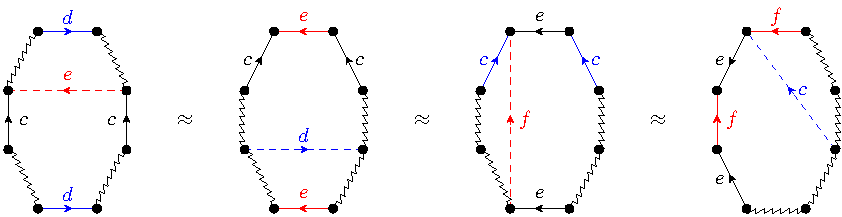
\includegraphics[width=1\linewidth]{H28.pdf}
		\caption{\small\textit{\color{duongvaotoanhoc}Hình $28$: Thay $2$ cặp cạnh $\{c,c^{-1}\}$ và $\{d,d^{-1}\}$ bởi dãy $efe^{-1}f^{-1}$.}}
		\vspace*{-10pt}
	\end{figure}
	Lặp lại Bước $4$ cho đến khi các cặp cạnh dạng $\{c,c^{-1}\}$ được phân hoạch vào cách dãy dạng $efe^{-1}f^{-1}$ (các cặp cạnh dạng $\{b,b\}$ vẫn luôn kề nhau). Ký hiệu thu được mô tả tổng liên thông của một số hữu hạn các mặt xuyến và các mặt phẳng xạ ảnh (mặt xuyến có ký hiệu là $aba^{-1}b^{-1}$ và mặt phẳng xạ ảnh có ký hiệu là $aa$. Vì tính giao hoán của tổng liên thông, ta có $X \approx \mathbb{T}^{\# m} \# \mathbb{P}^{\# n}$, với $m,n \in \mathbb{N}$. Nếu $m=0$ hoặc $n = 0$ thì chứng minh kết thúc. Trong trường hợp $m,n > 0$, ta áp dụng kết quả $\mathbb{T} \# \mathbb{P} \approx \mathbb{P}^3$ (ở cuối mục trước) $m$ lần liên tiếp để thu được $X \approx \mathbb{P}^{\# (2m + n)}$.
	\vskip 0.1cm
	Để chứng minh phần ``duy nhất'' của định lý chính, ta cần chỉ ra rằng các mặt đã liệt kê đôi một không đồng phôi. Một việc có thể làm ngay lúc này là chỉ ra rằng các mặt $\mathbb{P}^{\# g}$ (với $g > 0$) không đồng phôi với các mặt $\mathbb{T}^{\# h}$ (với $h \ge 0$, nhắc lại rằng $\mathbb{T}^0 := \mathbb{S}$). Thật vậy, mặt cầu và mặt xuyến là mặt một phía là các mặt hai phía (vì thế, các mặt xuyến với $h$ quai cầm, $h > 0$, cũng vậy) nên ta chỉ cần chỉ ra rằng rằng $\mathbb{P}^{\# g}$ là mặt một phía với mọi $g > 0$. Thật vậy
	\vskip 0.1cm
	$\bullet$ với $g = 1,2$, ta biết rằng $\mathbb{P}$ và $\mathbb{P} \# \mathbb{P} \approx \mathbb{K}$ (xem Hình $19$) là các mặt một phía, vì chúng đều chứa băng M\"obius (xem Hình $17$);
	\vskip 0.1cm
	$\bullet$ với $g \ge 3$ và chẵn thì $g = 2n$ (với $n \ge 2$), áp dụng liên tiếp kết quả $\mathbb{P}^{\# 3} \approx \mathbb{T} \# \mathbb{P}$, ta có $\mathbb{P}^{\# 2n} \approx \mathbb{T}^{n-1} \# \mathbb{P}^{\# 2} \approx \mathbb{T}^{n-1} \# \mathbb{K}$ là mặt một phía (vì $\mathbb{T}^{n-1}$ là mặt hai phía còn $\mathbb{K}$ là mặt một phía);
	\vskip 0.1cm	
	$\bullet$ với $g \ge 3$ và lẻ thì $g = 2n+1$ (với $n \ge 1$), tương tự, ta có $\mathbb{P}^{\#(2n+1)} \approx \mathbb{T}^n \# \mathbb{P}$ là mặt một phía (vì $\mathbb{T}^{n}$ là mặt hai phía còn $\mathbb{P}$ là mặt một phía).
	\vskip 0.1cm
	Phần còn lại của chứng minh cho tính duy nhất sẽ được hoãn lại tới mục sau, nơi ta giới thiệu thêm một bất biến tôpô quan trọng khác.
	\vskip 0.1cm
	$\pmb{6.}$ \textbf{\color{duongvaotoanhoc}Đặc trưng Euler--Poincar\'e. Giống}
	\vskip 0.1cm
	Cho $X$ là một mặt đóng và $\mathscr{T}$ là một phép tam giác phân hữu hạn của $X$. Lần lượt ký hiệu bởi $V(\mathscr{T})$, $E(\mathscr{T})$ và $F(\mathscr{T})$ số đỉnh, số cạnh và số tam giác cong trong $\mathscr{T}$. Số nguyên
	\begin{align*}
		\chi(\mathscr{T}) = V(\mathscr{T}) - E(\mathscr{T}) + F(\mathscr{T})
	\end{align*}
	là {\it đặc trưng Euler--Poincar\'e} của $\mathscr{T}$. Ta sẽ dùng giá trị này để chỉ ra rằng $\mathbb{S}$ không đồng phôi với $\mathbb{T}^m$ với $m > 0$ và rằng $\mathbb{T}^m$ không đồng phôi với $\mathbb{T}^n$ cũng như $\mathbb{P}^m$ không đồng phôi với $\mathbb{P}^n$ với $m \neq n$. Trước hết, ta cần chỉ ra rằng giá trị $\chi$ là một bất biến tôpô chỉ phụ thuộc vào nội tại mặt $X$, không phụ vào phép tam giác phân $\mathscr{T}$. Trong tôpô đại số, điều này được chứng minh nhờ khái niệm {\it lý thuyết đồng điều} và một tính toán đơn giản trên các {\it số Betti}. 
	\vskip 0.1cm
	Ở mục này, chúng ta cố gắng phác thảo một chứng minh không chính thức cho sự kiện này. Ý tưởng như sau, cho $\mathscr{T}$ và $\mathscr{T}'$ là hai tam giác phân tùy ý, ta dùng một số hữu hạn các phép biến đổi bảo toàn đặc trưng Euler--Poincar\'e để đưa $\mathscr{T}$ về $\mathscr{T}'$. Để làm điều này một cách thuận tiện, ta đưa ra một khái niệm tổng quát hơn tam giác phân: Ta gọi một {\it cấu trúc phân ngăn} trên $X$ là một họ $\mathscr{C}$ gồm một số hữu hạn các điểm, các đường và các đa giác cong trên $X$, thỏa mãn các tính chất sau.
	\vskip 0.1cm
	$\bullet$ Phần trong của mỗi đa giác cong đều đồng phôi với đĩa mở $\mathbb{D}$ và đôi một không giao nhau.
	\vskip 0.1cm
	$\bullet$ Biên của mỗi đa giác cong là hợp của một số hữu hạn các đường (ta gọi các đường này là các {\it cạnh} của đa giác cong, các đầu mút của chúng là các {\it đỉnh} của đa giác cong).
	\vskip 0.1cm
	$\bullet$ Sau khi bỏ điểm đầu và điểm cuối, các đường đều đồng phôi với khoảng mở $(0,1)$ và đôi một không giao nhau.
	\vskip 0.1cm
	Khái niệm trên cho phép sự xuất hiện của các đường với điểm đầu trùng với điểm cuối (các {\it khuyên}), các đa giác có thể có số cạnh tùy ý (thậm chí có thể bằng $1$ hoặc $2$), xem Hình $29$.
	\begin{figure}[H]
		\vspace*{-5pt}
		\centering\captionsetup{labelformat=empty, justification=centering}
		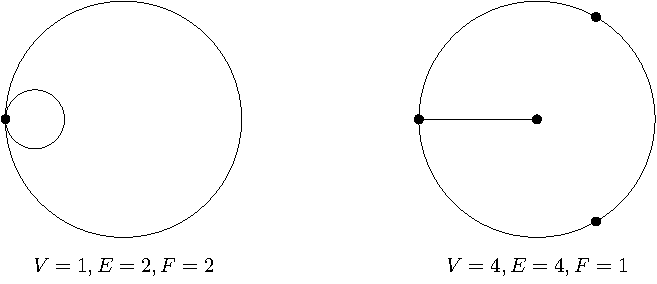
\includegraphics[width=1\linewidth]{H29.pdf}
		\caption{\small\textit{\color{duongvaotoanhoc}Hình $29$: Hai cấu trúc phân ngăn khác nhau của đĩa đóng.}}
		\vspace*{-10pt}
	\end{figure}
	Lần lượt ký hiệu bởi $V(\mathscr{C})$, $E(\mathscr{C})$ và $F(\mathscr{C})$ số điểm, số đường và số đa giác cong trong $\mathscr{C}$. Gọi
	\begin{align*}
		\chi(\mathscr{C}) = V(\mathscr{C}) - E(\mathscr{C}) + F(\mathscr{C})
	\end{align*}
	là đặc trưng Euler--Poincar\'e của $\mathscr{C}$. Dễ thấy các thao tác sau đây không làm thay đổi đặc trưng Euler--Poincar\'e của cấu trúc phân ngăn.
	\vskip 0.1cm
	$\bullet$ Chia đôi một đường bằng cách thêm một điểm vào giữa đường (số điểm và số đường đều tăng thêm $1$, số đa giác cong không đổi).
	\vskip 0.1cm	
	$\bullet$ Chia đôi một đa giác cong bằng cách thêm một đường nối hai đỉnh {\it không nhất thiết phân biệt} (số điểm không đổi, số đường và số đa giác cong đều tăng thêm $1$).
	\vskip 0.1cm	
	$\bullet$ Thêm một điểm ở miền trong của một đa giác cong và một đường nối nó với một đỉnh của đa giác (số điểm và số đường đều tăng thêm $1$, số đa giác cong không đổi).
	\vskip 0.1cm
	Giả sử $\mathscr{C}$ và $\mathscr{C}'$ là hai cấu trúc phân ngăn sao sao cho giao của mỗi đường của $\mathscr{C}$ với mỗi đường của $\mathscr{C}'$ chỉ gồm một số hữu hạn các điểm và một số hữu hạn các đoạn đóng. Khi đó ta có thể dùng một số hữu hạn các phép biến đổi trên để đưa $\mathscr{C}$ và $\mathscr{C}'$ về cùng một cấu trúc phân ngăn $\mathscr{C}''$, chẳng hạn như trong Hình $30$. Vì thế, ta có $\chi(\mathscr{C}) = \chi(\mathscr{C}'') = \chi(\mathscr{C}')$.
	\begin{figure}[H]
		\vspace*{-5pt}
		\centering\captionsetup{labelformat=empty, justification=centering}
		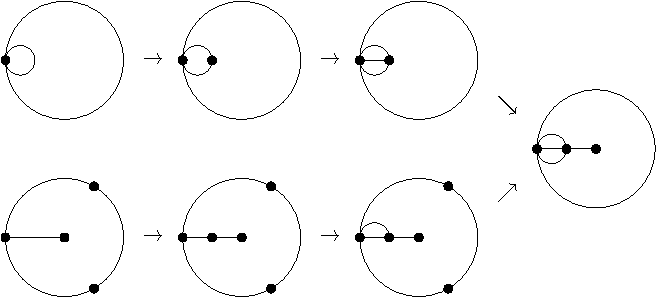
\includegraphics[width=1\linewidth]{H30.pdf}
		\caption{\small\textit{\color{duongvaotoanhoc}Hình $30$: Đưa hai cấu trúc phân ngăn ở Hình $29$ về cùng một cấu trúc phân ngăn.}}
		\vspace*{-10pt}
	\end{figure}
	Trường hợp xấu có thể xảy ra là khi giao của một đường trong $\mathscr{C}$ với một đường trong $\mathscr{C}'$ gồm một số vô hạn điểm hoặc một số vô hạn đoạn đóng. Lúc này, ta cần ``xê dịch'' hai đường này một chút để đưa về trường hợp trước. Đây là một bước rất kỹ thuật và cần dùng đến tính compact trong tôpô học, ta sẽ không đi sâu vào chi tiết.
	\vskip 0.1cm
	Từ các phân tích ở trên, ta có thể định nghĩa đặc trưng Euler--Poincar\'e $\chi(X)$ của một mặt đóng $X$ là đặc trưng Euler--Poincar\'e $\chi(\mathscr{T})$ của bất kỳ phép tam giác phân hữu hạn $\mathscr{T}$ (hoặc bất kỳ cấu trúc phân ngăn hữu hạn $\mathscr{C}$) nào của $X$. Chẳng hạn, mặt xuyến có một tam giác phân $\mathscr{T}$ cho bởi Hình $13$, với $V(\mathscr{T}) = 9$, $E(\mathscr{T}) = 27$ và $F(\mathscr{T}) = 18$, nên $\chi(\mathbb{T}) = 9 - 27 + 18 = 0$. Một phép đồng phôi biến một tam giác phân của mặt này thành một tam giác phân của mặt kia, với số đỉnh, số cạnh và số tam giác cong được bảo toàn. Vì thế, hai mặt đồng phôi có cùng đặc trưng Euler--Poincar\'e, nghĩa là đặc trưng Euler--Poincar\'e là một bất biến tôpô.
	\vskip 0.1cm
	Cho $X$ và $Y$ là các mặt đóng, ta tìm công thức liên hệ giữa $\chi(X \# Y)$ với $\chi(X)$ và $\chi(Y)$ như sau. Xét $\mathscr{T},\mathscr{T}'$ lần lượt là các tam giác phân hữu hạn bất kỳ của $X$ sao cho có ít nhất một tam giác cong $T \in \mathscr{T}$ nằm trong $X^\circ$ và ít nhất một tam giác cong $T' \in \mathscr{T}'$ nằm trong $Y^\circ$. Ta khoét $T^{\circ}$ và $T'^{\circ}$ khỏi $X$ và $Y$ rồi dán $X \setminus T^\circ$ với $Y \setminus T'^{\circ}$ dọc theo $\partial T \approx \partial T'$ để thu được tổng liên thông $X \# Y$. Có $3$ đỉnh được dán lại với nhau, $3$ cạnh được dán lại với nhau, và $2$ tam giác cong bị bỏ đi, do đó tam giác phân mới thu được trên $X\#Y$ gồm $V(\mathscr{T}) + V(\mathscr{T}') - 3$ đỉnh, $E(\mathscr{T}) + E(\mathscr{T}') - 3$ cạnh và $F(\mathscr{T}) + F(\mathscr{T}') - 2$ tam giác cong. Từ đó ta tính được
	\begin{align*}
		\chi(X \# Y) = \chi(X) + \chi(Y) - 2.
	\end{align*}
	Thay $Y = \mathbb{S}$ trong công thức trên (nhắc lại rằng $X \# \mathbb{S} \approx X$), ta thu được $\chi(\mathbb{S}) = 2$. Mặt khác, bằng quy nạp, ta dễ dàng tính được
	\begin{align*}
		\chi(X^{\# g}) = g \cdot \chi(X) + 2 - 2g
	\end{align*}
	với $g \ge 1$. Từ đó ta có $\chi(\mathbb{T}^{\# g}) = 2-2g \le 0$. Do đó, mặt $\mathbb{S}$ cùng các mặt $\mathbb{T}^g$, với $g \ge 1$, đôi một không đồng phôi (nhắc lại rằng tất cả các mặt này đều là mặt hai phía).
	\vskip 0.1cm
	Ngoài ra, từ kết quả $\mathbb{P} \# \mathbb{T} \approx \mathbb{P}^{\# 3}$, ta tính được $\chi(\mathbb{P}) = 1$, suy ra $\chi(\mathbb{T}^{\# g}) = 2-g$. Do đó, các mặt $\mathbb{P}^g$, với $g \ge 1$, đôi một không đồng phôi (nhắc lại rằng tất cả các mặt này đều là mặt một phía). Điều này kết thúc chứng minh của định lý phân loại tôpô cho các mặt đóng.
	\vskip 0.1cm
	Ta kết thúc bài viết bằng việc nhắc đến khái niệm sau đây. Với $X$ là một mặt đóng, nếu $X$ là mặt hai phía thì tồn tại duy nhất số tự nhiên $g$ sao cho $\chi(X) = 2-2g$, hay $X \approx \mathbb{T}^{\#g}$ (nhắc lại quy ước $\mathbb{T}^{\# 0} = \mathbb{S}$). Số tự nhiên $g$ này được gọi là {\it giống} (genus) của mặt $X$, nó chính là ``số quai cầm'' của $X$ (mặt cầu không có quai cầm, tổng liên thông $\mathbb{T}^{\# g}$ có $g$ quai cầm). Theo tinh thần này, nếu $X$ là mặt một phía thì tồn tại duy nhất số nguyên dương $g$ sao cho $\chi(X) = 2-g$ (ta có $X \approx \mathbb{P}^{\# g}$). Ta cũng gọi $g$ là giống của $X$ trong trường hợp này (một số nơi gọi số nguyên này là {\it á giống}). Định lý chính của bài viết này nói rằng, mặt đóng $X$ được xác định duy nhất (sai khác đồng phôi) khi ta biết tính khả định hướng và giống của nó.
\end{multicols}